% SC4040 --- Chapter 6: Advanced String Algorithms (0->100 ground-up)
\chapter{Advanced String Algorithms}
\label{ch:string-adv}

\begin{quote}
\emph{``Text is not just characters --- it is structure waiting to be indexed.''}
From suffix arrays to the Burrows--Wheeler transform and the FM-index, this chapter builds compressed full-text indexes from first principles.
\end{quote}

\noindent\fbox{\parbox{\dimexpr\linewidth-2\fboxsep-2\fboxrule}{%
\textbf{From zero: strings as arrays.} We define alphabets, suffixes, and lexicographic order before any index. No prior string-algorithms beyond naive search assumed.}}
\vspace{0.4em}

\section*{Learning Outcomes}
After this chapter you will be able to:
\begin{enumerate}[label=(L\arabic*)]
    \item define suffix arrays and construct them in $O(n\log n)$ via doubling/prefix-doubling;
    \item compute the LCP array (Kasai) and use it for $O(m+\log n)$ pattern search and LCE queries;
    \item define the Burrows--Wheeler transform and prove LF-mapping invertibility;
    \item build the FM-index (rank + LF) for $O(m)$ counting and locating in compressed space;
    \item analyse space/time trade-offs among suffix arrays, suffix trees, BWT, and FM-index.
\end{enumerate}

% ============================================================
\section{Suffix Arrays: Sorting All Suffixes}
\label{sec:suffix-array}

For $T[0\ldots n-1]$ with sentinel $T[n-1]=\$$ smaller than all letters, suffix $S_i=T[i\ldots n-1]$. The \emph{suffix array} $\text{SA}[0\ldots n-1]$ is the permutation with $S_{\text{SA}[0]}<\cdots<S_{\text{SA}[n-1]}$ lexicographically.

\begin{figure}[h]\centering
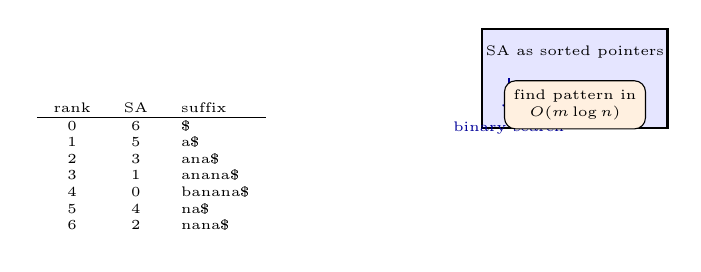
\begin{tikzpicture}[scale=0.84,font=\scriptsize]
\node[font=\tiny,align=left] at (0,0) {
\begin{tabular}{ccl}
rank & SA & suffix\\\hline
0&6&\$\\
1&5&a\$\\
2&3&ana\$\\
3&1&anana\$\\
4&0&banana\$\\
5&4&na\$\\
6&2&nana\$
\end{tabular}};
\begin{scope}[xshift=5cm,yshift=0.6cm]
\draw[thick,fill=blue!10] (0,0) rectangle (2.8,1.5);
\node[font=\tiny,align=center] at (1.4,1.15) {SA as sorted pointers};
\draw[->,thick,blue!60!black] (0.4,0.75)--(0.4,0.25) node[below,font=\tiny] {binary search};
\node[draw,rounded corners,fill=orange!12,font=\tiny,align=center] at (1.4,0.35) {find pattern in\\$O(m\log n)$};
\end{scope}
\end{tikzpicture}
\caption{Suffix array of \texttt{banana\$}. Sorted suffixes enable binary search for any pattern; LCP accelerates to $O(m+\log n)$.}
\label{fig:suffix-array}
\end{figure}

\textbf{Doubling construction ($O(n\log n)$):} rank suffixes by first $2^k$ characters. Initially rank by single character. To double, sort pairs $(\text{rank}_k[i],\text{rank}_k[i+2^k])$ via radix sort; re-rank. After $\lceil\log n\rceil$ rounds, ranks are distinct and equal SA order. Each round is $O(n)$ radix sort, total $O(n\log n)$.

\begin{lstlisting}[language=Python]
def suffix_array(s):
    """Doubling O(n log n) suffix array. s: string with sentinel."""
    n = len(s)
    k = 1
    rank = [ord(c) for c in s]
    sa = list(range(n))
    tmp = [0]*n
    while True:
        sa.sort(key=lambda x: (rank[x], rank[x+k] if x+k<n else -1))
        tmp[sa[0]] = 0
        for i in range(1, n):
            prev, cur = sa[i-1], sa[i]
            tmp[cur] = tmp[prev] + ((rank[prev], rank[prev+k] if prev+k<n else -1) <
                                     (rank[cur],  rank[cur+k]  if cur+k<n  else -1))
        rank, tmp = tmp, rank
        if rank[sa[-1]] == n-1: break
        k <<= 1
    return sa

def lcp_kasai(s, sa):
    """Kasai O(n) LCP array. lcp[i]=lcp(sa[i], sa[i-1])."""
    n = len(s); rank = [0]*n
    for i, p in enumerate(sa): rank[p] = i
    lcp, h = [0]*n, 0
    for i in range(n):
        r = rank[i]
        if r == 0: continue
        j = sa[r-1]
        while i+h < n and j+h < n and s[i+h]==s[j+h]: h+=1
        lcp[r]=h
        if h: h-=1
    return lcp
\end{lstlisting}

LCP array plus RMQ gives $O(1)$ longest-common-extension queries, powering $O(m+\log n)$ pattern search via two binary searches with LCP-guided comparisons.

% ============================================================
\section{Burrows--Wheeler Transform: Reversible Permutation}
\label{sec:bwt}

Form all rotations of $T$, sort them, take last column $L$ (and first column $F$ which is just sorted characters). $L$ is the BWT. Key property: equal characters in $F$ and $L$ correspond via LF-mapping, so $T$ is recoverable from $L$ alone.

\begin{figure}[h]\centering
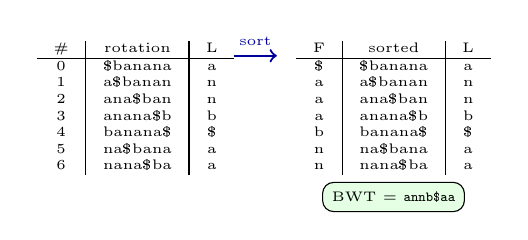
\begin{tikzpicture}[scale=0.78,font=\scriptsize]
\node[font=\tiny,align=left] at (0,0) {
\begin{tabular}{c|c|c}
\#& rotation & L\\\hline
0&\$banana & a\\
1&a\$banan & n\\
2&ana\$ban & n\\
3&anana\$b & b\\
4&banana\$ & \$\\
5&na\$bana & a\\
6&nana\$ba & a
\end{tabular}};
\draw[->,thick,blue!60!black] (1.6,0.85)--(2.3,0.85) node[midway,above,font=\tiny] {sort};
\node[font=\tiny,align=left] at (4.2,0) {
\begin{tabular}{c|c|c}
F & sorted & L\\\hline
\$&\$banana & a\\
a&a\$banan & n\\
a&ana\$ban & n\\
a&anana\$b & b\\
b&banana\$ & \$\\
n&na\$bana & a\\
n&nana\$ba & a
\end{tabular}};
\node[draw,rounded corners,fill=green!10,font=\tiny] at (4.2,-1.45) {BWT = \texttt{annb\$aa}};
\end{tikzpicture}
\caption{BWT of \texttt{banana\$}: sort rotations, read last column. Runs in $L$ cluster equal contexts, enabling compression; LF-mapping inverts it.}
\label{fig:bwt}
\end{figure}

\begin{definition}[LF-mapping]
Let $C[c]=\#\{j:T[j]<c\}$ and $\text{rank}_c(i)=\#\{j\le i:L[j]=c\}$. If $L[i]=c$ is the $k$-th $c$ in $L$, its position in $F$ is $C[c]+k$. Formally $\text{LF}(i)=C[L[i]]+\text{rank}_{L[i]}(i)$.
\end{definition}

Inversion: start at row with $\$$, repeatedly apply LF to recover $T$ backwards in $O(n)$.

\begin{lstlisting}[language=Python]
def bwt_via_sa(s):
    """BWT from suffix array. s must end with $."""
    sa = suffix_array(s); n = len(s)
    # L[i] = s[sa[i]-1] (char before suffix)
    return ''.join(s[sa[i]-1] if sa[i]>0 else s[-1] for i in range(n))

def inverse_bwt(L):
    """Invert BWT via LF-mapping. Returns original string."""
    n = len(L)
    # C[c]: count of chars < c
    chars = sorted(set(L))
    C = {}; cnt = 0
    for c in chars:
        C[c] = cnt; cnt += L.count(c)
    # rank via prefix counts
    occ = {c: [0]*(n+1) for c in chars}
    for i, ch in enumerate(L):
        for c in chars: occ[c][i+1] = occ[c][i] + (ch==c)
    def lf(i): return C[L[i]] + occ[L[i]][i+1] - 1  # 0-indexed subtlety: C is 0-based
    # find row with $
    row = L.index('$')
    res = []
    for _ in range(n):
        res.append(L[row])
        row = lf(row)
    return ''.join(reversed(res))
\end{lstlisting}

% ============================================================
\section{FM-Index: Search in Compressed Space}
\label{sec:fm-index}

The FM-index stores $L$ plus $\text{rank}$ structures ($O(n\log\sigma)$ bits) and supports:
\begin{itemize}
    \item \textbf{Count} occurrences of $P$ ($|P|=m$) in $O(m)$ via backward search: maintain interval $[lo,hi)$ of rows prefixed by suffix of $P$; update $lo=C[c]+\text{rank}_c(lo)$, $hi=C[c]+\text{rank}_c(hi)$.
    \item \textbf{Locate} positions by sampling SA entries and walking LF.
    \item \textbf{Extract} substrings via LF walks from sampled positions.
\end{itemize}

\begin{figure}[h]\centering
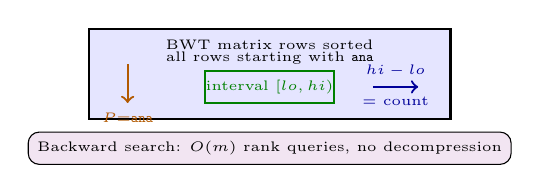
\begin{tikzpicture}[scale=0.82,font=\scriptsize]
\draw[thick,fill=blue!10] (0,0) rectangle (5.6,1.4);
\node[font=\tiny] at (2.8,1.15) {BWT matrix rows sorted};
\draw[->,thick,orange!70!black] (0.6,0.85)--(0.6,0.25) node[below,font=\tiny] {$P$=\texttt{ana}};
\draw[thick,green!50!black] (1.8,0.75) rectangle (3.8,0.25) node[midway,font=\tiny] {interval $[lo,hi)$};
\node[font=\tiny] at (2.8,0.95) {all rows starting with \texttt{ana}};
\draw[->,thick,blue!60!black] (4.4,0.5)--(5.1,0.5) node[midway,above,font=\tiny] {$hi-lo$} node[midway,below,font=\tiny] {= count};
\node[draw,rounded corners,fill=violet!10,font=\tiny] at (2.8,-0.45) {Backward search: $O(m)$ rank queries, no decompression};
\end{tikzpicture}
\caption{FM-index backward search: each character of $P$ (right-to-left) narrows the BWT interval. Final width equals occurrence count.}
\label{fig:fm-index}
\end{figure}

Space is close to empirical entropy $nH_k$ plus lower-order terms; with wavelet trees, $\text{rank}_c$ is $O(\log\sigma)$ per query, often $O(1)$ for small alphabets.

% ============================================================
\section{Worked Example: FM-index Count Trace}
\label{sec:fm-trace}

$T=\texttt{banana\$}$, BWT $L=\texttt{annb\$aa}$, $C[\$]=0,C[a]=1,C[b]=4,C[n]=5$. Search $P=\texttt{ana}$ backwards: start $[0,7)$, $c=\texttt{a}$ gives $[1,4)$, next $\texttt{n}$ gives $[5,7)$, next $\texttt{a}$ gives $[2,3)$ of width $1$ --- exactly one occurrence at SA position $3$ (suffix \texttt{anana\$}).

% ============================================================
\section{Suffix Trees vs.\ Suffix Arrays}
\label{sec:suffix-tree}

Suffix trees store the same information as suffix arrays plus LCP but with $O(n)$ nodes and heavier constants (Ukkonen $O(n)$ online construction). Suffix arrays with LCP are often faster in practice due to cache locality and smaller memory ($4n$ vs.\ $20n$ bytes). Enhanced suffix arrays (Abouelhoda et al.) simulate tree traversals via SA+LCP+child table, combining best of both.

% ============================================================
\section{Chapter Notes}
Suffix arrays (Manber--Myers 1993) and Kasai et al.\ (2001) LCP are textbook staples (Gusfield). Burrows--Wheeler (1994) underpins bzip2; Ferragina--Manzini (2000) created the FM-index. SA-IS (Nong et al.\ 2009) builds SA in linear time; FM-index variants power Bowtie/BWA aligners.

% ============================================================
\section{Exercises}
\label{sec:ch06-exercises}
\begin{enumerate}[label=E6.\arabic*, leftmargin=*, itemsep=0.7em]
    \item \textbf{Doubling correctness.} Prove the doubling step: if suffixes are sorted by first $2^k$ characters, sorting pairs $(\text{rank}_k[i],\text{rank}_k[i+2^k])$ sorts by first $2^{k+1}$ characters. Deduce $O(n\log n)$ total time with radix sort.
    \item \textbf{LCP binary search.} Show how LCP + RMQ accelerates pattern search from $O(m\log n)$ to $O(m+\log n)$: maintain lcp with interval endpoints and skip known matching prefix.
    \item \textbf{LF is a permutation.} Prove LF is a bijection on $[0,n-1]$ and that iterating LF from the $\$$ row recovers $T$ backwards. Illustrate on \texttt{abracadabra\$}.
    \item \textbf{FM-index count.} Trace backward search for $P=\texttt{ana}$ on BWT \texttt{annb\$aa} of \texttt{banana\$}. Give $[lo,hi)$ after each character.
    \item \textbf{Locate via sampling.} Suppose every $s$-th SA entry is stored. Show locating all $\text{occ}$ occurrences costs $O(s\cdot\text{occ})$ LF steps. How to choose $s$ to balance space vs.\ time?
\end{enumerate}
% End of Chapter 6
